% TanitAD-4B: hierarchical latent world models with typed abstraction interfaces
% Self-contained LaTeX source (pdfLaTeX). Figures are TikZ / pgfplots, drawn in the source.
\documentclass[10pt,twocolumn]{article}

\usepackage[a4paper,margin=18mm,columnsep=7mm,top=20mm,bottom=22mm]{geometry}
\usepackage[T1]{fontenc}
\usepackage[utf8]{inputenc}
\usepackage{amsmath,amsthm,mathtools}
\usepackage{newtxtext,newtxmath}
\usepackage{bm}
\usepackage[protrusion=true]{microtype}
\usepackage{booktabs,tabularx,multirow,array}
\usepackage{xcolor}
\usepackage{tikz}
\usetikzlibrary{arrows.meta,positioning,fit,backgrounds,calc,shapes.geometric,decorations.pathreplacing}
\usepackage{pgfplots}
\pgfplotsset{compat=1.18}
\usepackage[font=small,labelfont=bf,labelsep=period]{caption}
\usepackage{enumitem}
\setlist{nosep,leftmargin=1.2em}
\usepackage[colorlinks=true,linkcolor=navy,citecolor=navy,urlcolor=navy]{hyperref}
\usepackage[capitalise,nameinlink]{cleveref}

% ---------------------------------------------------------------- colours of the hierarchy levels
\definecolor{navy}{HTML}{1B2A41}
\definecolor{levS}{HTML}{B04A86}
\definecolor{levT}{HTML}{1F6FB2}
\definecolor{levO}{HTML}{C98500}
\definecolor{levF}{HTML}{3A7D5C}
\definecolor{enc}{HTML}{56636F}
\definecolor{soft}{HTML}{F3F5F8}

\newtheorem{proposition}{Proposition}
\newtheorem{definition}{Definition}
\theoremstyle{remark}
\newtheorem{remark}{Remark}

\newcommand{\Rset}{\mathbb{R}}
\newcommand{\ADE}{\mathrm{ADE}}
\newcommand{\tier}[1]{\textsc{\small #1}}

\tikzset{
  box/.style={draw=#1,very thick,rounded corners=2pt,fill=#1!8,minimum height=7mm,align=center,font=\footnotesize},
  plain/.style={draw=enc,thick,rounded corners=2pt,fill=soft,minimum height=7mm,align=center,font=\footnotesize},
  arr/.style={-{Stealth[length=2.2mm]},thick},
  goal/.style={-{Stealth[length=2.2mm]},very thick},
  lat/.style={-{Stealth[length=2.2mm]},thick,dashed},
  lbl/.style={font=\scriptsize,align=center,text=navy},
}

\title{\vspace{-6mm}\textbf{TanitAD-4B: Hierarchical Latent World Models with Typed Abstraction Interfaces\\for Data-Efficient Autonomous Driving}}
\author{Dr.-Ing.\ Sayed Bouzouraa\\[1mm]\normalsize TanitAD Research}
\date{November 2026}

\makeatletter
\renewcommand\paragraph{\@startsection{paragraph}{4}{\z@}{1.6ex \@plus .5ex \@minus .2ex}{-1em}{\normalfont\normalsize\bfseries}}
\makeatother
\raggedbottom
\begin{document}
\maketitle

% =====================================================================================================================
\begin{abstract}
End-to-end driving models have won the architecture argument, yet they remain data-hungry, opaque, unaware of their own limits and
expensive at inference time. We present \emph{TanitAD-4B}, a programme that attacks all four weaknesses with one design principle:
\emph{drive at every level of abstraction, and make every level accountable}. The 4B architecture factorises driving into four
brains (operative, tactical, strategic and fallback), each with its own clock, horizon, state space and predictor. The operative
level owns up to 2\,s, the tactical level up to 6\,s and the strategic level 6 to 30\,s. Every level reads the current measured ego state.
The tactical level emits goals and constraints that act as the action conditioning the operative level, and the output is one
trajectory or several, up to 6\,s. Goals condition strictly downward and latents flow upward through stop-gradient barriers. We describe the self-supervised world-model objective
behind the programme (residual multi-horizon latent prediction, provable anti-collapse via sliced Epps--Pulley regularisation,
inverse dynamics and calibrated imagination of unobserved areas) and its current reference implementation, \emph{v8F-mini}.
v8F-mini makes the hierarchy \emph{typed}: route checkpoints, a 60-dimensional tactical code of goals, manoeuvres and continuous
constraints, and a trajectory that is an exact residual on a frozen learned kinematic prior. With only 7.2\,M trainable parameters,
trained in four hours on one 8\,GB consumer GPU, it reduces 6\,s displacement error against its learned kinematic floor by
0.31/0.43\,m at two training seeds in open loop. A zero-training post-map makes it better than that floor on \emph{every} row of a
pre-registered metric set. Driving on its own executed motion, the adopted model lowers 6\,s error by 1.26/1.19\,m and improves at
least one row in each of the four metric families: longitudinal, lateral, tactical and strategic (a measurement; the strategic bars are paused by decision). Split by horizon band, on-policy (DAgger) data carries the 2--6\,s band and an acceleration-matching term the 0--2\,s band; a per-band loss with the operative level detached from the tactical one adds a reproduced 0--2\,s gain, and the tactical level's top three manoeuvres contain the logged one in 90\,\% of windows. Oracle reads place 87--89\,\% of the remaining tactical headroom in the tactical level's continuous constraints, chiefly target speed, and its sharpest cause in missed stop decisions: the operative level executes a correct stop (1.5\,m lower tactical error on stop-point windows), while loss re-weighting only moves the stop decision along one ROC curve, so the next lever is stop perception. We also state the design as nine theorems with measurable premises and check them by machine (56 solver conditions and 54 Lean~4 theorems). They give the exact conditions under which a multi-level predictor and a decision-first planner dominate their flat counterparts, and a pooling theorem: a world-model state that averages over image cells keeps counts and totals and loses position and motion. Measured on the trained model, that state holds the presence of a lead vehicle beyond ego motion (AUROC 0.81/0.79 against 0.60) and nothing about how its gap changes; the hierarchy is ahead of a flat control on selection-critical windows, and the comparison on all windows is not yet established. All of it rests on an evaluation
doctrine built for decisions rather than leaderboards: pre-registered bars with both outcomes committed, episode-cluster bootstrap
intervals, explicit seed variance and four metric families on every evaluation. We close with the remaining frontier (assertive
launch from standstill), the re-rendered simulation tier built to address it, and a research roadmap toward a 4B driver within a
budget of at most 800\,M parameters, deployable within 100\,ms on an edge computer.
\end{abstract}

% =====================================================================================================================
\section{Introduction}
Driving is a hierarchy of decisions on separated time scales. A route is chosen over tens of seconds, a manoeuvre with its
parameters over seconds, a control profile over tenths of a second. Monolithic end-to-end planners collapse this structure into one
mapping from pixels to waypoints. That buys simplicity and gives up four things a production driver needs:
\begin{itemize}
  \item \textbf{data efficiency}, because every situation must be learned jointly at every scale;
  \item \textbf{inspectability}, because no intermediate decision is exposed;
  \item \textbf{self-knowledge}, because nothing in the model says when it is outside its competence;
  \item \textbf{efficient inference}, because the full network runs at the control rate.
\end{itemize}

TanitAD is a research programme built on the opposite bet. A driver should \emph{imagine} the consequences of its options in a
learned latent world model, at the level of abstraction where each decision lives, and expose each level's decision as a typed,
measurable interface. We call the architecture \emph{4B}, for its four brains:
\begin{itemize}
  \item an \textbf{operative} brain for continuous control and the trajectory, up to 6\,s;
  \item a \textbf{tactical} brain that emits goals and constraints up to 6\,s;
  \item a \textbf{strategic} brain for route checkpoints, detected context and the goals derived from them, over 6 to 30\,s;
  \item a \textbf{fallback} brain that monitors the others and owns the minimal-risk manoeuvre.
\end{itemize}

\paragraph{Contributions.}
\begin{enumerate}[label=(\roman*)]
  \item \textbf{The 4B formalism} (\cref{sec:4b}): per-level predictors in shrinking state spaces at slowing clocks, downward goal
        conditioning, and a gradient-isolation matrix that is \emph{checked} rather than assumed.
  \item \textbf{v8F-mini} (\cref{sec:v8f}), a typed three-level instantiation over frozen foundation features:
        \begin{itemize}
          \item a tactical code with 22 goals, 12 manoeuvre classes and 26 continuous constraints;
          \item a trajectory parameterisation in which a zero residual reproduces a learned kinematic prior \emph{exactly}, so every
                learned metre is measured against the floor.
        \end{itemize}
  \item \textbf{Mathematical analysis} (\cref{sec:math}): a Lipschitz decomposition of plan error into an oracle term and propagated
        interface errors, the convex response of the operative layer to tactical accuracy, why whole-code teacher forcing leaves
        partial codes unsupported, and a three-variance account of evaluation intervals.
  \item \textbf{A machine-checked theory} (\cref{sec:theory,sec:premises}): nine statements on when a hierarchy, a pooled state, a
        rule shield, imagination and weight averaging can and cannot help, checked by an SMT solver and the Lean~4 kernel, each
        with a premise that is then measured.
  \item \textbf{Results under a decision-grade doctrine} (\cref{sec:eval,sec:results}): improvements over the kinematic floor in open
        loop and on the model's own executed motion, with at least one improved row in each of the four metric families.
  \item \textbf{A roadmap} (\cref{sec:frontier,sec:outlook}): re-rendered simulation on neural reconstructions, perception adaptation,
        and scaling toward the 4B budget of at most 800\,M parameters.
\end{enumerate}

% =====================================================================================================================
\section{Related work}
\paragraph{Hierarchical latent world models.} 
\begin{itemize}
  \item H-JEPA~\cite{hjepa} stacks action-conditioned joint-embedding predictive models that predict further ahead in coarser latents,
        with top-down sub-goal planning.
  \item Hierarchical planning with latent world models~\cite{hplwm} reports large gains of two-level sub-goals over flat planners at
        matched capacity.
  \item In driving, Orbis~2~\cite{orbis2}, Drive-HWM~\cite{drivehwm} and S2Planner~\cite{s2planner} apply hierarchical or multi-scale
        world models on NAVSIM~\cite{navsim}.
\end{itemize}
TanitAD differs in making the hierarchy a \emph{supervised typed interface} whose usage is measured by intervention.

\paragraph{Self-supervised representations.} 
\begin{itemize}
  \item DINOv3~\cite{dinov3} supplies frozen visual features.
  \item V-JEPA~2~\cite{vjepa2} and LeJEPA~\cite{lejepa} motivate latent prediction with isotropic-Gaussian regularisation.
  \item LoRA~\cite{lora} is the adaptation route of our perception outlook.
\end{itemize}

\paragraph{Why modularity can help.} Shalev-Shwartz and Shashua~\cite{ssshashua} show a sample-complexity separation in favour of
semantic-abstraction training, under an assumption of approximately independent module failures, which our interface analysis
addresses directly.

\paragraph{Exposure bias and on-policy data.} Scheduled sampling~\cite{schedsamp}, DAgger~\cite{dagger}, DART~\cite{dart}, causal
confusion~\cite{causalconf} and the limits of behaviour cloning~\cite{bclimits} frame the mismatch between a consumer trained on
ground truth and one fed its predecessor's output.

\paragraph{End-to-end planners.} 
\begin{itemize}
  \item Representative designs: conditional imitation~\cite{cil}, ChauffeurNet~\cite{chauffeurnet}, TransFuser~\cite{transfuser},
        VAD~\cite{vad}, Hydra-MDP~\cite{hydramdp}, DiffusionDrive~\cite{diffusiondrive} and residual planners~\cite{resad}.
  \item They are evaluated on nuPlan~\cite{nuplan} and NAVSIM~\cite{navsim}.
\end{itemize}

% =====================================================================================================================
\section{The 4B architecture}\label{sec:4b}

\begin{figure*}[t]
\centering
\resizebox{0.96\textwidth}{!}{%
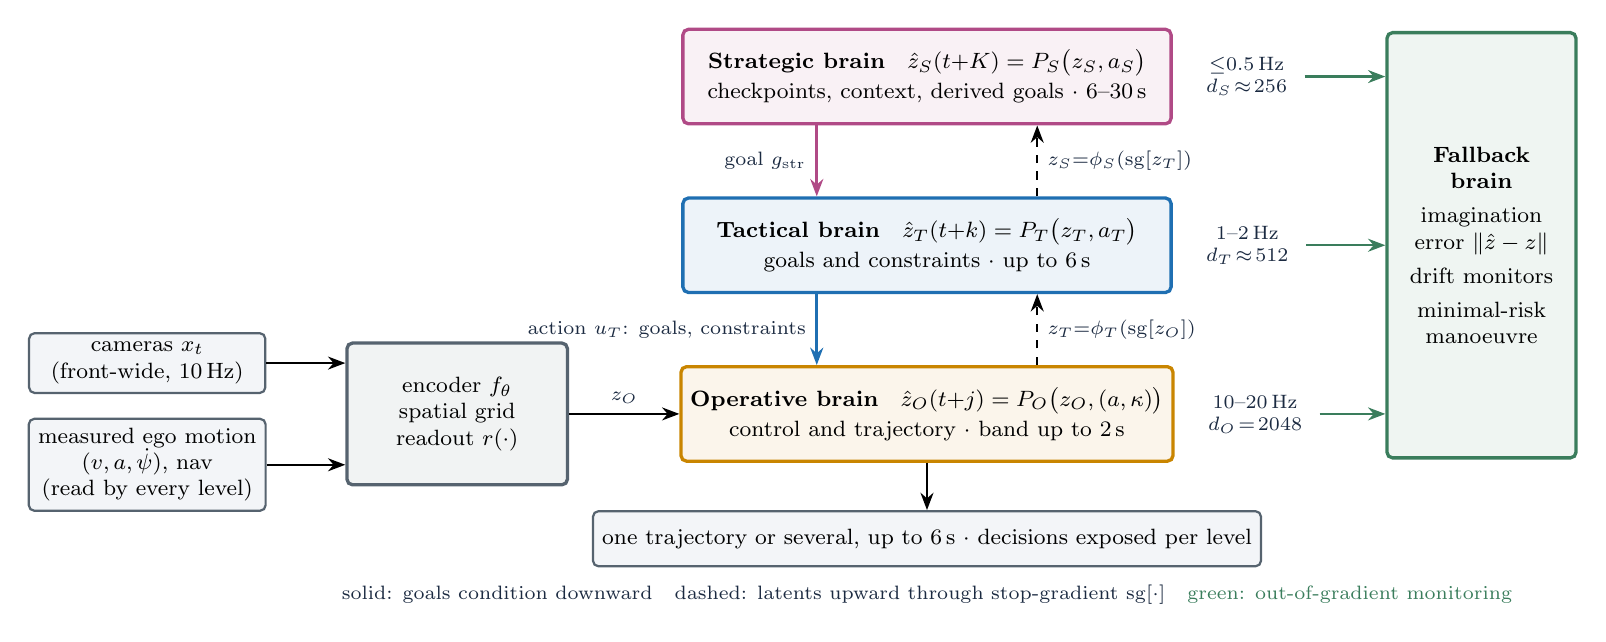
\begin{tikzpicture}[node distance=4mm and 6mm]
  % sensors and encoder
  \node[plain,minimum width=30mm] (cam) {cameras $x_t$\\(front-wide, 10\,Hz)};
  \node[plain,minimum width=30mm,below=3mm of cam] (ego) {measured ego motion\\$(v,a,\dot\psi)$, nav\\(read by every level)};
  \node[box=enc,minimum width=28mm,minimum height=18mm,right=10mm of $(cam.east)!0.5!(ego.east)$] (enc) {encoder $f_\theta$\\spatial grid\\readout $r(\cdot)$};
  \draw[arr] (cam.east) -- (enc.west|-cam.east);
  \draw[arr] (ego.east) -- (enc.west|-ego.east);
  % the three predictive brains
  \node[box=levO,minimum width=62mm,minimum height=12mm,right=14mm of enc] (O) {\textbf{Operative brain} \; $\hat z_O(t{+}j)=P_O\big(z_O,(a,\kappa)\big)$\\[0.5mm] control and trajectory $\cdot$ band up to 2\,s};
  \node[box=levT,minimum width=62mm,minimum height=12mm,above=9mm of O] (T) {\textbf{Tactical brain} \; $\hat z_T(t{+}k)=P_T\big(z_T,a_T\big)$\\[0.5mm] goals and constraints $\cdot$ up to 6\,s};
  \node[box=levS,minimum width=62mm,minimum height=12mm,above=9mm of T] (S) {\textbf{Strategic brain} \; $\hat z_S(t{+}K)=P_S\big(z_S,a_S\big)$\\[0.5mm] checkpoints, context, derived goals $\cdot$ 6--30\,s};
  \draw[arr] (enc.east) -- node[lbl,above]{$z_O$} (O.west);
  % clocks
  \node[lbl,right=3mm of S] (cS) {$\le$0.5\,Hz\\$d_S\!\approx\!256$};
  \node[lbl,right=3mm of T] (cT) {1--2\,Hz\\$d_T\!\approx\!512$};
  \node[lbl,right=3mm of O] (cO) {10--20\,Hz\\$d_O\!=\!2048$};
  % goals down (solid), latents up (dashed, stop-gradient)
  \draw[goal,levS] ([xshift=-14mm]S.south) -- node[lbl,left]{goal $g_{\mathrm{str}}$} ([xshift=-14mm]T.north);
  \draw[goal,levT] ([xshift=-14mm]T.south) -- node[lbl,left]{action $u_T$: goals, constraints} ([xshift=-14mm]O.north);
  \draw[lat] ([xshift=14mm]O.north) -- node[lbl,right]{$z_T{=}\phi_T(\mathrm{sg}[z_O])$} ([xshift=14mm]T.south);
  \draw[lat] ([xshift=14mm]T.north) -- node[lbl,right]{$z_S{=}\phi_S(\mathrm{sg}[z_T])$} ([xshift=14mm]S.south);
  % fallback brain
  \node[box=levF,minimum width=24mm,minimum height=54mm,right=27mm of T,yshift=0mm] (F) {\textbf{Fallback}\\\textbf{brain}\\[1mm]imagination\\error $\|\hat z-z\|$\\[1mm]drift monitors\\[1mm]minimal-risk\\manoeuvre};
  \draw[arr,levF] (S.east -| cS.east) ++(1mm,0) -- (F.west|-S.east);
  \draw[arr,levF] (T.east -| cT.east) ++(1mm,0) -- (F.west|-T.east);
  \draw[arr,levF] (O.east -| cO.east) ++(1mm,0) -- (F.west|-O.east);
  % output
  \node[plain,below=6mm of O,minimum width=62mm] (plan) {one trajectory or several, up to 6\,s $\cdot$ decisions exposed per level};
  \draw[arr] (O.south) -- (plan.north);
  % legend
  \node[lbl,below=1mm of plan,align=left] {\textcolor{navy}{solid: goals condition downward}\quad \textcolor{navy}{dashed: latents upward through stop-gradient $\mathrm{sg}[\cdot]$}\quad \textcolor{levF}{green: out-of-gradient monitoring}};
\end{tikzpicture}}
\caption{\textbf{The 4B architecture.} Four brains at separated clocks and horizons. Each predictive level owns its own predictor in
its own latent space, and the state shrinks while the clock slows going up ($d_S<d_T<d_O$, $\tau_S>\tau_T>\tau_O$), so upper levels
are forced to abstract. Goals condition strictly downward, through the readers and the planner cost; the predictors themselves are action-conditioned and goal-free. Latents pass upward only through stop-gradient adapters, and the
gradient-isolation matrix of \cref{eq:gmatrix} is tested on every build. The fallback brain consumes every level's imagination error
and owns the minimal-risk manoeuvre.}
\label{fig:4b}
\end{figure*}

\subsection{Levels, clocks and predictors}
Let $\ell\in\{O,T,S\}$ index the operative, tactical and strategic levels. Each level owns:
\begin{itemize}
  \item a state $z_\ell\in\Rset^{d_\ell}$;
  \item a clock $\tau_\ell$ and a horizon;
  \item an action space $a_\ell$;
  \item a predictor $P_\ell$ in its own space.
\end{itemize}
The operative state is a spatial-grid readout of the encoder, $z_O=r(f_\theta(x))$ (never a global pool). Upper states are adapters over
\emph{stopped} lower latents, $z_T=\phi_T(\mathrm{sg}[z_O])$ and $z_S=\phi_S(\mathrm{sg}[z_T])$. Each level's dynamics are conditioned on
that level's own action:
\begin{equation}
\begin{aligned}
\hat z_S(t{+}K) &= P_S\big(z_S(t),a_S(t)\big),\\
\hat z_T(t{+}k) &= P_T\big(z_T(t),a_T(t)\big),\\
\hat z_O(t{+}j) &= P_O\big(z_O(t),(a,\kappa)_t\big).
\end{aligned}
\end{equation}
Goals do not enter the predictors. They condition the lower levels through the readers and the planner cost (\cref{sec:bands}).
Two structural properties follow by construction and are then verified.

\paragraph{(1) Abstraction by down-sampling under a shrinking state.} With $d_S<d_T<d_O$ and $\tau_S>\tau_T>\tau_O$, an upper level cannot
represent lower-level detail even if its objective would reward it. At 0.2\,Hz a 15\,s strategic roll is three steps of a 256-dimensional
model (about seven at 0.5\,Hz), so only the operative path runs at the full rate.

\paragraph{(2) The gradient-isolation matrix.} Let $G[u,v]=1$ iff a gradient path from module $u$ into module $v$ is permitted. With
$\mathcal P$ the planner and goal heads and $\mathcal E$ the encoder,
\begin{equation}\label{eq:gmatrix}
G[\mathcal P,\mathcal E]=0,\quad G[\ell',\ell]=0\ \ (\ell'\text{ above }\ell),\quad G[\ell,\ell]=1 .
\end{equation}
Every build checks it by asserting zero gradient on forbidden paths, with a deliberate-regression arm that must fail.

\subsection{Time bands, the current ego state and the tactical action}\label{sec:bands}
Let $\Delta=0.2$\,s be the grid step and $t$ the present. The levels own the bands
\begin{equation}
B_O=(0,2]\,\mathrm{s},\quad B_T=(2,6]\,\mathrm{s},\quad B_S=(6,30]\,\mathrm{s}.
\end{equation}
The output of the stack is one trajectory or several, up to 6\,s,
\begin{equation}
X_t=\big(x_{t+j\Delta}\big)_{j=1}^{30}\in\Rset^{30\times2},
\end{equation}
so knots 1--10 lie in $B_O$ and knots 11--30 in $B_T$. A horizon of 0.8\,s is not a long-term abstract level: a level's reach has to
match its band.

\paragraph{The cascade.} Let $e_t$ be the current measured ego state, including yaw rate, and $V_t$ the vision tokens of the current and
past frames, with the navigation command and speed limit. Every level reads $e_t$, and no level reads a state planned by another level:
\begin{equation}\label{eq:cascade}
\begin{aligned}
s_t&=f_S(e_t,V_t),\\
u_t&=f_T(e_t,V_t,\hat s),\\
X_t&=f_O(e_t,V_t,\hat s,\hat u),
\end{aligned}
\end{equation}
where a hat marks a held output re-expressed in the current ego frame by measured odometry. The tactical output is a \emph{tactical
action},
\begin{equation}
u_t=(g_t,\lambda^{\mathrm{lat}}_t,\lambda^{\mathrm{lon}}_t,\gamma_t),
\end{equation}
the goals, the lateral and longitudinal classes and the constraints, over a horizon of up to 6\,s. T has no trajectory head. $u_t$
conditions O as its action, so the plan is a function of the context \emph{given} $u_t$. A single decoder produces all 30 knots, which
makes the plan continuous across 2\,s by construction, and the two bands differ only in the loss:
\begin{equation}
\mathcal L_O=w_{\mathrm{op}}\,\ell\big(X^{1:10},X^{\ast\,1:10}\big)+w_{\mathrm{tac}}\,\ell\big(X^{11:30},X^{\ast\,11:30}\big).
\end{equation}
For $M$ hypotheses, $X^{(m)}_t=f_O(\,\cdot\mid\hat u^{(m)})$ with $\hat u^{(m)}$ the $M$ best tactical actions; $M=1$ is the arm of record.

\paragraph{The strategic level.} Its output is $\sigma_t=(C_t,p_t,\gamma^S_t)$: checkpoints $C_t$ at $\tau\in\{6,9,\dots,30\}$\,s; the
posteriors $p_t$ of the detected context (country, period of day, illumination, weather, visibility and road surface), read from the
current and past images only; and the goals $\gamma^S_t$ derived from them. $\sigma_t$ enters $f_T$ as a detached input, so strategic goals
reach O through $u_t$. No output of a situation classifier enters any goal path.

\paragraph{World-model planning.} The levels $l=1,2,3$ step at $\tau_l=0.2,0.6,3.0$\,s and are trained to reaches of 2, 6 and 18\,s. Following
H-JEPA~\cite{hjepa}, with $g$ a goal latent, $\tilde z^{\,l+1}_i$ the rollout of level $l$ lifted to the level above, and $l=2,1$,
\begin{equation}
\begin{aligned}
a^{3,\ast}&=\arg\min_{a^3}\big\|\hat z^{\,3}_{T_3}-g\big\|^2,\\
a^{l,\ast}&=\arg\min_{a^l}\big\|\tilde z^{\,l+1}_{K}-\hat z^{\,l+1,\ast}_{K}\big\|^2\\
&\qquad+\lambda\sum_{i<K}\big\|\tilde z^{\,l+1}_{i}-\hat z^{\,l+1,\ast}_{i}\big\|^2 .
\end{aligned}
\end{equation}
Each level plans from its own encoded current state, and the only downward signal is the predicted state of the level above. This
planner is the baseline against which other approaches are compared.

\paragraph{Status.} \Cref{eq:cascade} is trained on v8F-mini as described in \cref{sec:v8f}, with equal knot weights and tactical labels
over 2--8\,s. The band losses, the 2--6\,s labels, the strategic extension and the world-model planner are built and tested, and the
world models for these bands are in training. A first planner read on the earlier models, with a true-future goal (T0), did not beat
holding the action. No driving result exists yet for this design.

\subsection{Self-supervised world-model objective}
The programme's world model is trained without perception labels, without HD maps and without reward. Its objective is
\begin{equation}
\begin{aligned}
\mathcal L={}&\mathcal L_{\mathrm{pred}}+\lambda_{\mathrm{tac}}\mathcal L_{\mathrm{tac}}+\lambda_{\mathrm{sig}}\big(\mathcal S(Z)+\mathcal S(\hat Z)\big)\\
&+\lambda_{\mathrm{inv}}\mathcal L_{\mathrm{inv}}+\lambda_{\mathrm{im}}\mathcal L_{\mathrm{imag}} .
\end{aligned}
\end{equation}
\paragraph{Residual multi-horizon prediction.} $\hat z_{t+k}=z_t+\Delta_k(z_{t-W+1:t},a_{t-W+1:t})$, scored by a \emph{change-weighted}
error with per-dimension weights $w\propto|z_{t+k}-z_{t+k-1}|$ normalised to unit mean. On driving data only 5--11\,\% of a frame
changes per step, so the weighting puts the gradient where the consequences are.

\paragraph{Provable anti-collapse.} $\mathcal S(\cdot)$ is the sliced Epps--Pulley statistic of LeJEPA~\cite{lejepa}. Embeddings are
projected onto $M$ fresh unit directions, and each projection $Y$ (a sample of size $n$) is tested against $\mathcal N(0,1)$:
\begin{equation}
T_{n,\beta}=\tfrac1n\!\sum_{j,k}e^{-\frac{\beta^2(Y_j-Y_k)^2}{2}}-\tfrac{2}{\sqrt{1+\beta^2}}\sum_j e^{-\frac{\beta^2Y_j^2}{2(1+\beta^2)}}+\tfrac{n}{\sqrt{1+2\beta^2}} .
\end{equation}
By the Cram\'er--Wold theorem, standard normal one-dimensional projections in all directions imply a joint standard Gaussian, the
embedding law LeJEPA shows to be optimal; $M$ random directions test this only approximately. The gradients stay uniformly bounded~\cite{lejepa}.

\paragraph{Inverse dynamics.} $\mathcal L_{\mathrm{inv}}=\|g(z_t,z_{t+1})-a_t\|^2$ uses proprioception as free supervision and forces
controllable state into the latent.

\paragraph{Imagination of unobserved areas.} Masked sectors evolve by semi-Lagrangian advection under a learned flow,
$\hat z_{t+1}(u)=z_t(u-v_\theta(u)\Delta t)$, refined by attention, with a per-cell log-variance $s(u)$:
\begin{equation}
\mathcal L_{\mathrm{imag}}=\sum_u w(u)\Big[e^{-s(u)}\tfrac{\|\hat z(u)-z(u)\|^2}{2}+\tfrac{s(u)}{2}\Big],
\end{equation}
with $w=1$ on hidden cells and 0.1 on visible ones. The model must know \emph{where it cannot know}. The variance field is the
world-model-native trigger for sensor steering and for the fallback brain.

\subsection{Why a hierarchy is data-efficient}
Two arguments motivate the factorisation~\cite{hplwm,ssshashua}.
\begin{enumerate}[label=(\roman*)]
  \item \textbf{Horizon.} Planning regret in learned models grows with the horizon, so a short per-level horizon has a smaller bound at
        that level. Summed over the levels, equal per-step errors give the undivided bound back: the gain requires the coarser levels
        to carry a smaller per-step error, which is an empirical question.
  \item \textbf{Recombination.} If a driving situation is a combination of a place $p\in\mathcal P$, a manoeuvre $m\in\mathcal M$ and a
        control profile, a flat learner must cover $|\mathcal P|\cdot|\mathcal M|$ combinations. A hierarchy that learns each level
        separately covers roughly $|\mathcal P|+|\mathcal M|$, provided places and manoeuvres combine independently.
\end{enumerate}

\subsection{Fallback and self-knowledge}
The relative imagination error $\|\hat z_t-z_t\|$ is a free, always-on familiarity signal. Layered monitors arm a deterministic
minimal-risk manoeuvre:
\begin{itemize}
  \item imagination error at 10\,Hz;
  \item routing statistics at 1\,Hz;
  \item Mahalanobis drift at 0.1\,Hz.
\end{itemize}
Their logs are the substrate for the ISMR/DSSAD incident-reporting requirements: self-monitoring \emph{is} the evidence trail.

The programme's 263\,M-parameter 4B flagship was its first arm to beat the kinematic floor in open loop: ADE@2\,s 0.452\,m against
0.500\,m for the best of three kinematic models and 0.523\,m for CTRV. On windows where kinematics diverge from the realised future, it
beat CTRV by 0.80\,m, and the whole of that advantage came from vision.

% =====================================================================================================================
\section{v8F-mini: a typed reference implementation}\label{sec:v8f}

\begin{figure*}[t]
\centering
\resizebox{0.98\textwidth}{!}{%
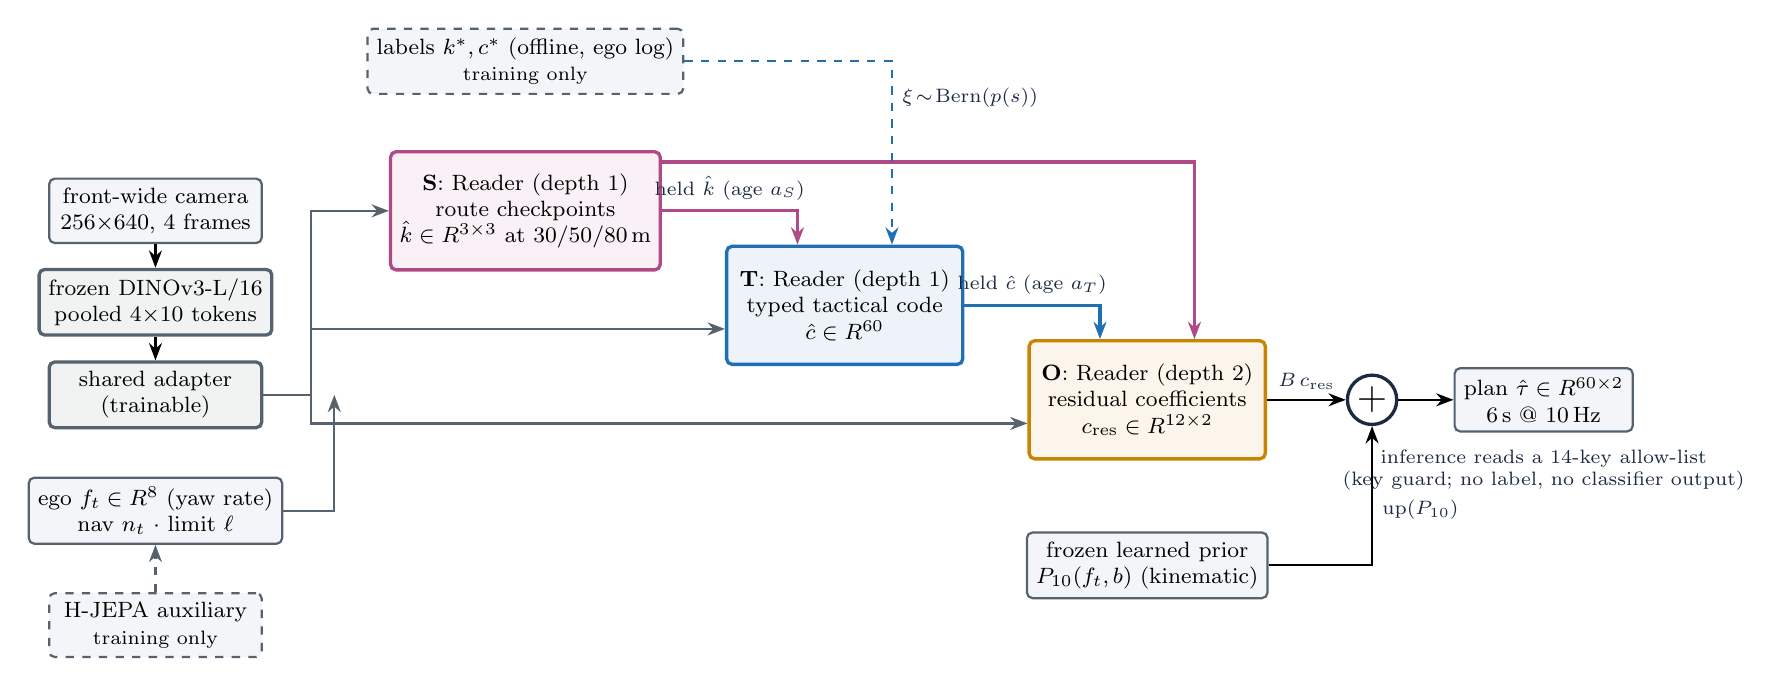
\begin{tikzpicture}[node distance=5mm and 7mm]
  % inputs
  \node[plain,minimum width=27mm] (img) {front-wide camera\\256$\times$640, 4 frames};
  \node[box=enc,minimum width=27mm,below=3mm of img] (dino) {frozen DINOv3-L/16\\pooled $4{\times}10$ tokens};
  \node[box=enc,minimum width=27mm,below=3mm of dino] (adp) {shared adapter\\(trainable)};
  \node[plain,minimum width=27mm,below=6mm of adp] (ego) {ego $f_t\in\Rset^8$ (yaw rate)\\nav $n_t$ $\cdot$ limit $\ell$};
  \draw[arr] (img) -- (dino); \draw[arr] (dino) -- (adp);
  % readers
  \node[box=levS,minimum width=30mm,minimum height=15mm,right=16mm of img] (S) {\textbf{S}: Reader (depth 1)\\route checkpoints\\$\hat k\in\Rset^{3\times3}$ at 30/50/80\,m};
  \node[box=levT,minimum width=30mm,minimum height=15mm,right=8mm of S,yshift=-12mm] (T) {\textbf{T}: Reader (depth 1)\\typed tactical code\\$\hat c\in\Rset^{60}$};
  \node[box=levO,minimum width=30mm,minimum height=15mm,right=8mm of T,yshift=-12mm] (O) {\textbf{O}: Reader (depth 2)\\residual coefficients\\$c_{\mathrm{res}}\in\Rset^{12\times2}$};
  \coordinate (bus) at ($(adp.east)+(6mm,0)$);
  \draw[thick,enc] (adp.east) -- (bus);
  \draw[arr,enc] (bus) |- (S.west);
  \draw[arr,enc] (bus) |- ([yshift=-3mm]T.west);
  \draw[arr,enc] (bus) |- ([yshift=-3mm]O.west);
  \draw[arr,enc] (ego.east) -| ([xshift=3mm]bus);
  % held outputs flow down the hierarchy
  \draw[goal,levS] (S.east) -| node[lbl,above,pos=0.25]{held $\hat k$ (age $a_S$)} ([xshift=-6mm]T.north);
  \draw[goal,levT] (T.east) -| node[lbl,above,pos=0.25]{held $\hat c$ (age $a_T$)} ([xshift=-6mm]O.north);
  \draw[goal,levS] ([yshift=-1.5mm]S.north east) -| ([xshift=6mm]O.north);
  % prior and sum
  \node[plain,minimum width=30mm,below=9mm of O] (P10) {frozen learned prior\\$P_{10}(f_t,b)$ (kinematic)};
  \node[circle,draw=navy,very thick,inner sep=1.2pt,right=10mm of O] (sum) {\Large$+$};
  \node[plain,right=7mm of sum,minimum width=22mm] (tau) {plan $\hat\tau\in\Rset^{60\times2}$\\6\,s @ 10\,Hz};
  \draw[arr] (O.east) -- node[lbl,above]{$B\,c_{\mathrm{res}}$} (sum.west);
  \draw[arr] (P10.east) -| node[lbl,right,pos=0.7]{$\mathrm{up}(P_{10})$} (sum.south);
  \draw[arr] (sum.east) -- (tau.west);
  % training-only components
  \node[plain,dashed,minimum width=30mm,above=7mm of S] (lab) {labels $k^\ast,c^\ast$ (offline, ego log)\\\scriptsize training only};
  \draw[lat,levT] (lab.east) -| node[lbl,right,pos=0.6]{\scriptsize $\xi\!\sim\!\mathrm{Bern}(p(s))$} ([xshift=6mm]T.north);
  \node[plain,dashed,minimum width=27mm,below=6mm of ego] (wm) {H-JEPA auxiliary\\\scriptsize training only};
  \draw[lat,enc] (wm.north) -- (ego.south);
  % guard
  \node[lbl,below=1mm of tau,align=center] (guard) {\textcolor{navy}{inference reads a 14-key allow-list}\\\textcolor{navy}{(key guard; no label, no classifier output)}};
\end{tikzpicture}}
\caption{\textbf{v8F-mini.} Three learned readers over frozen DINOv3 features and a shared trainable adapter. S emits route checkpoints,
T a typed 60-dimensional tactical code, and O the coefficients of a ramped cosine basis added to a \emph{frozen} learned kinematic
prior. Upper outputs are \emph{held} with quantised ages and re-expressed in the current frame by odometry. Labels enter only through
scheduled teacher forcing in training. Inference reads a fixed allow-list of inputs, enforced by a key guard.}
\label{fig:v8f}
\end{figure*}

\subsection{Inputs and notation}
Time runs on a 0.2\,s grid. For a window ending at $t$, the model reads:
\begin{itemize}
  \item \textbf{scene tokens} $z_{t'}\in\Rset^{40\times1024}$, frozen DINOv3-L/16 features of the cylindrical front-wide frame, pooled to a
        $4\times10$ grid, four frames per layer;
  \item \textbf{ego features} $f_t=(v,a,\kappa,v^2,va,v\kappa,v^2\kappa,a\kappa)$, with curvature $\kappa$ from the \emph{measured yaw rate}
        (never a steering angle);
  \item \textbf{a navigation command} $n_t$;
  \item \textbf{a speed bucket} $\ell$;
  \item \textbf{measured odometry} between frames.
\end{itemize}
The output is a 6\,s plan $\tau\in\Rset^{60\times2}$ in the ego frame, scored on its 30 knots at 0.2\,s. Several plans are possible,
one per top tactical hypothesis; the arm reported here emits one.

\subsection{The S/T/O decomposition}
S ticks at about 1\,Hz, T at about 2\,Hz and O at 10\,Hz. On the cache grid the model uses sample-and-hold with quantised ages:
\begin{itemize}
  \item T last ticked $a_T\in\{0,1,2\}$ steps ago;
  \item S ticked $u\le4$ steps before T, so $a_S=a_T+u$.
\end{itemize}
With $t_T=t-a_T$ and $t_S=t-a_S$,
\begin{equation}
\begin{aligned}
\hat k&=f_S\big(z_{t_S},f_{t_S},n_{t_S},\ell\big),\\
\hat c&=f_T\big(z_{t_T},f_{t_T},n_{t_T},\ell,\Pi_{t_S\to t_T}\hat k\big),\\
\hat\tau&=f_O\big(z_t,f_t,n_t,\ell,\Pi_{t_S\to t}\hat k,\hat c,(a_T,a_S)\big),
\end{aligned}
\end{equation}
where $\Pi_{a\to b}$ re-expresses held checkpoints from frame $a$ to frame $b$ by odometry. The conditioning sets are strictly nested,
$\mathrm{in}(S)\subset\mathrm{in}(T)\subset\mathrm{in}(O)$. Information flows between levels only through \emph{held outputs}, never
through shared hidden state. Each level reads the measured ego state of its own tick, and no level reads a state planned by another
level. Each $f_\ell$ is a \emph{Reader}: four learned queries cross-attend to the conditioning and scene tokens
through a pre-norm transformer decoder, followed by an MLP head.

\subsection{The tactical code as a typed interface}
\begin{equation}
\begin{aligned}
c=\big[\,&\underbrace{\sigma(g)}_{22\text{ goals}}\;\big|\;\underbrace{\mathrm{softmax}(\lambda_{\mathrm{lat}})}_{5}\;\big|\\
&\underbrace{\mathrm{softmax}(\lambda_{\mathrm{lon}})}_{7}\;\big|\;\underbrace{(\gamma-\mu)/\sigma_{\mathrm{cons}}}_{26\text{ constraints}}\,\big]\in\Rset^{60}.
\end{aligned}
\end{equation}
The 26 constraint cells cover turn timing and geometry, longitudinal target speeds and reach times, the stop point, the lead gap and
time gap, and the speed band. The code is the tactical action of \cref{sec:bands}: T emits goals and constraints, has no trajectory
head, and $\hat c$ conditions O. The route checkpoints of this arm sit at 30, 50 and 80\,m, with a median arrival of 3, 5 and 8\,s, so
they do not yet cover the strategic band in seconds; \cref{sec:bands} gives the extension.

\paragraph{An information-theoretic reading.} Ground-truth codes $C^\ast=g(Y)$ are deterministic functions of the human future $Y$, so the
data-processing inequality gives $I(C;Y)\ge I(C;C^\ast)$. Supervised agreement with $C^\ast$ is therefore a lower-bound proxy for
informativeness about the future. O also reads the scene, so the code is a \emph{typed side channel}, not a strict bottleneck, and its
usage is measurable by intervention (\cref{sec:results}).

\subsection{Trajectory as an exact residual on a kinematic prior}
Let $P=P_{10}(f_t,b)\in\Rset^{30\times2}$ be a \emph{frozen} learned prior: a damped base path re-timed by constant acceleration, plus an
eight-feature MLP fitted once. Let $\mathrm{up}$ interpolate it to 0.1\,s. The plan is
\begin{equation}\label{eq:traj}
\tau=\mathrm{up}\big(P_{10}(f_t,b)\big)+B\,c_{\mathrm{res}},\quad B_{ik}=\tfrac{i+1}{N}\cos\!\Big(\tfrac{k\pi(i+\frac12)}{N}\Big),
\end{equation}
with $N=60$, $k=0,\dots,11$, $c_{\mathrm{res}}=s\cdot\mathrm{MLP}(h_O)$, $s=2$\,m, and the last layer zero-initialised.

\begin{proposition}[Floor identity, ramp and band limit]\hfill
\begin{enumerate}[label=(\alph*)]
  \item \textbf{Floor identity.} $c_{\mathrm{res}}=0$ implies $\tau=\mathrm{up}(P_{10})$ exactly, so the untrained model \emph{is} the prior.
  \item \textbf{Ramp.} $|B_{ik}|\le(i+1)/N$, so the residual vanishes linearly as $t\to0$ and the plan starts at the prior's origin.
  \item \textbf{Band limit.} With $k\le11$ the cosine factor has at most eleven half-cycles over 6\,s, below 1\,Hz, and the linear ramp
        modulates it smoothly: a smooth adjustment, while the prior carries the kinematics.
\end{enumerate}
\end{proposition}
Every learned metre is thus measured against the floor it must beat. Each property is pinned by a unit test with a mutation check.

\subsection{Losses and scheduled teacher forcing}
The training loss is
\begin{multline}
\mathcal L=w_{\mathrm{ck}}\mathcal L_{\mathrm{ck}}+w_{\mathrm{tac}}\big(\mathcal L_{\mathrm{goal}}+\tfrac12(\mathcal L_{\mathrm{lat}}+\mathcal L_{\mathrm{lon}})+w_{\mathrm{cons}}\mathcal L_{\mathrm{cons}}\big)\\
+w_{\mathrm{traj}}\big(\tfrac13\mathcal L_{\ADE}+\tfrac1{12}\mathcal L_{\mathrm{FDE}}\big)+w_{\mathrm{pen}}\textstyle\sum_r\rho_r+w_{\mathrm{wm}}\mathcal L_{\mathrm{wm}}.
\end{multline}
Its terms:
\begin{itemize}
  \item \textbf{partial-label cross-entropies} $-\log\sum_{c\in\mathcal A}p_c$ handle the sets of allowed manoeuvres;
  \item \textbf{constraint cells} use a masked Huber loss;
  \item \textbf{rule penalties} $\rho_r$ (speed, stop, turn, lead) are differentiable hinges that are positive \emph{iff} a frozen rule reports a
        violation;
  \item \textbf{the world-model auxiliary} $\mathcal L_{\mathrm{wm}}$ is an H-JEPA objective on the shared adapter~\cite{hjepa}.
\end{itemize}
During training, O and T read a mixture of predicted and ground-truth upper outputs,
\begin{equation}
\begin{gathered}
\tilde c=\xi_c\,c^\ast+(1-\xi_c)\,\hat c,\qquad \xi_c\sim\mathrm{Bernoulli}\big(p(s)\big),\\
p(s)=1-0.8\min(s/S,1),
\end{gathered}
\end{equation}
which anneals the share of ground truth from 1.0 to 0.2~\cite{schedsamp}. At inference $\xi\equiv0$, and labels are never read.

\subsection{Admissibility by construction}
\begin{itemize}
  \item Inference reads a fixed allow-list of 14 keys. A key guard records every access during the forward pass, and a test proves
        that a deliberately peeking model is caught.
  \item The goal path may not contain the output of any situation classifier.
  \item Labels may use the ego future, but inference may not.
\end{itemize}

% =====================================================================================================================
\section{Mathematical background}\label{sec:math}

\subsection{Plug-in composition and propagated interface error}
By the chain rule, $p(y\mid x)=\sum_{k,c}p(k\mid x)\,p(c\mid x,k)\,p(y\mid x,k,c)$. Factorisation alone is an identity; its value lies in
\emph{supervision structure}. Each factor is fitted against its own offline target, and inference is a plug-in composition
$\hat y=\mu_O(x,\hat k,\hat c)$.
\begin{proposition}[Error decomposition]\label{prop:lip}
If $\mu_O$ is $L_k$- and $L_c$-Lipschitz in its code arguments, then
\begin{equation}
\begin{aligned}
\|\hat y-y\|\le{}&\underbrace{\|\mu_O(x,k^\ast,c^\ast)-y\|}_{\textup{oracle term}}\\
&+L_c\|\hat c-c^\ast\|+L_k\|\hat k-k^\ast\| .
\end{aligned}
\end{equation}
\end{proposition}
\noindent The oracle term is measurable by substituting ground-truth codes. The gap between the model's own code and the oracle is
the propagated interface error, and it is the headroom the hierarchy offers (\cref{sec:results}).

\subsection{Convex response to tactical accuracy}
Define the partial substitution $\hat c_\alpha=\hat c+\alpha(c^\ast-\hat c)$ on the 26 constraint cells, and the recovered fraction
\begin{equation}
r(\alpha)=\frac{\ADE(\hat c)-\ADE(\hat c_\alpha)}{\ADE(\hat c)-\ADE(\hat c_1)} .
\end{equation}
Linear response gives $r(\alpha)=\alpha$. We measure $r(0.25)=0.08$--$0.16$, $r(0.5)=0.20$--$0.36$ and $r(0.75)=0.48$--$0.73$. The
response is \emph{convex}: O is flat near its own code and steep near the truth. The value of tactical accuracy therefore compounds,
and the last metres of tactical precision buy the most driving.

\subsection{Interface support and exposure bias}
Whole-code teacher forcing trains O on the two-point mixture $p\,\delta_{c^\ast(x)}+(1-p)\,\delta_{\hat c(x)}$. A partial code
$c_u=(c^\ast_u,\hat c_{\bar u})$ lies off that support, so its response is unconstrained by the training loss. The remedy is to widen
the support: draw an independent $\xi_u$ per unit of the code at the same marginal $p(s)$,
\begin{equation}
\tilde c_u=\xi_u c^\ast_u+(1-\xi_u)\hat c_u,\qquad \xi_u\stackrel{\mathrm{iid}}{\sim}\mathrm{Bern}\big(p(s)\big).
\end{equation}
This keeps each cell's marginal unchanged while covering $2^7$ corners per window instead of 2.

The same logic applies along time. A policy trained only on expert states incurs compounding error of order $\varepsilon T^2$, while
on-policy aggregation (DAgger~\cite{dagger}) reduces it to order $\varepsilon T$ under that reduction's no-regret assumptions. v8F-mini realises this by replacing 10\,\% of the
training samples with the model's \emph{own rolled-out states}, labelled from the human future.

\subsection{Estimator theory: three variances, one interval}
Windows are grouped into $M=141$ episodes. For arms $a,b$ the point estimate is the full-set mean difference
$\hat\Delta=\frac1N\sum_w[d_a(w)-d_b(w)]$. The paired episode-cluster bootstrap resamples episodes with replacement, using the same
draw for both arms, and reports percentile intervals. By the law of total variance, with training randomness $\theta$, inference
randomness $\omega$ and the episode draw $E$,
\begin{equation}
\begin{aligned}
\mathrm{Var}(\hat\Delta)={}&\underbrace{\mathrm{Var}_\theta\,\mathbb E[\hat\Delta\mid\theta]}_{\text{training seeds}}+\underbrace{\mathbb E_\theta\mathrm{Var}_\omega\,\mathbb E_E[\hat\Delta\mid\theta,\omega]}_{\text{inference}}\\
&+\underbrace{\mathbb E_{\theta,\omega}\mathrm{Var}_E[\hat\Delta\mid\theta,\omega]}_{\text{episodes}} .
\end{aligned}
\end{equation}
The bootstrap estimates the episode term only. TanitAD therefore reports the seed term separately, through two training seeds and a
pre-registered floor $F=|\Delta_{s_0}-\Delta_{s_1}|$ with bar $2F$. For a deterministic forward pass the inference term is exactly zero,
and the programme verifies that on re-evaluation (maximum per-window deviation 0.0\,m).

% =====================================================================================================================
\section{A machine-checked theory of the hierarchy}\label{sec:theory}
The design claims of \cref{sec:4b} can be stated as theorems about model classes. Each has a premise that must be \emph{measured}
before it says anything about a model. We wrote nine such statements (T1--T9, \cref{tab:theory}) and froze each before its proof.
All were checked by machine: 56 verification conditions with the SMT solver Z3, each family with mutated twins that the solver must
refute (30 are), and the central ones in general form with the Lean~4 kernel and Mathlib (54 theorems, no \texttt{sorry}, standard
axioms only). Two groups were written after reads they explain; for those reads they are explanatory, not predictive. The premises
are tested in \cref{sec:premises}.

\begin{table*}[t]
\centering
\caption{\textbf{Nine statements, their machine check, and their measured premise for v8F-mini.} Z3: verification conditions proved by
an SMT solver, with mutated twins refuted. Lean: checked by the Lean~4 kernel in general form. Every measured value is a \tier{T0} or
\tier{T1-kin} diagnostic on logged frames, never driving performance (seed 0 / seed 1 where two values are given).}
\label{tab:theory}
\small
\begin{tabularx}{\textwidth}{@{}l>{\raggedright\arraybackslash}p{60mm}l>{\raggedright\arraybackslash}X@{}}
\toprule
 & Statement & Check & Measured premise or consequence for v8F-mini \\
\midrule
T1 & A level that jumps $k$ steps has the better worst-case bound at every horizon iff $\varepsilon_k<\varepsilon\sum_{i<k}L^i$ & Z3, Lean &
holds in the linear class: the direct 2\,s error is 0.42/0.43 of ten one-step errors; the learned ten-step rollout fails (skill $-0.15$/$-0.17$ at 2\,s) \\
T2 & Under squared error no plan beats the mean; under a hit-or-miss criterion a decided plan beats every single plan iff selection accuracy exceeds the share of the larger mode & Z3, Lean &
open: top-1 selection 57--59\,\%; the hierarchy is ahead of a flat control on selection-critical windows ($-0.48$/$-0.16$\,m) and not established on all windows \\
T3 & A shield keeps a rule for every network; a penalty of weight $\lambda$ only bounds the violation by $(J_0-J_\infty)/\lambda$ & Z3 &
with the logged rest distance: overrun exactly 0 and stop-window 2--6\,s ADE $-3.51$/$-3.37$\,m; with the model's own stop cue: no gain \\
T4 & Class weighting is a threshold move, $\tau=r/(1+r)$ & Z3 &
one added bias reproduces the stop decision of a class-weighted training run in 4 of 4 cells \\
T5 & A state pooled over cells keeps counts and totals and loses position and motion & Z3, Lean &
planted object: AUROC 1.00 from a grid state, 0.50 from the mean state; trained state: lead presence $+0.21$/$+0.19$ AUROC beyond ego motion, change of the gap: nothing beyond ego motion \\
T6 & Skill over persistence is the predictable fraction of the change & Z3 &
the learned world model is below a closed-form ridge at 0.2\,s and at 2\,s; a closed-form stack of both is above both at every horizon \\
T7 & An imagined gain is a real gain only above twice the model gap & Z3 &
not yet admissible for objects: the state decodes to the scene gist, and its learned rollout is no closer to the future than a copy \\
T8 & Sampling by gradient norm minimises the second moment of the weighted gradient & Z3 &
selection by coverage or by leverage lands inside the range of random draws (probe level); trained arms are running \\
T9 & A member average is never worse than the member mean; a rank-one edit is the least change that moves one key & Z3 &
a two-member weight average realises 0.74 of the ensemble gain in one forward pass \\
\bottomrule
\end{tabularx}
\end{table*}

\subsection{When multi-level prediction dominates}
Let a one-step predictor have error at most $\varepsilon$ and let the dynamics expand an error by at most the factor $L\ge0$ per
step, so that $e_{t+1}\le L\,e_t+\varepsilon$ with $e_0=0$.
\begin{proposition}[Composed bound, jump bound and criterion]\label{prop:jump}
After $H$ steps $e_H\le\varepsilon\sum_{i<H}L^{i}$, and the bound is attained. A level that predicts $k$ steps at once with error
$\varepsilon_k$ has error at most $\varepsilon_k\sum_{j<m}L^{kj}$ after $m$ jumps. At every horizon $H=mk$ with $m\ge1$, the jump bound
is below the composed bound if and only if
\begin{equation}
\varepsilon_k<\varepsilon\sum_{i<k}L^{i}\qquad(\text{for }L=1:\ \varepsilon_k<k\,\varepsilon).\label{eq:jump}
\end{equation}
\end{proposition}
\noindent The horizon drops out. A slow level earns its place exactly when its direct $k$-step error is below $k$ composed fast
steps. This is the formal content of the clocks of \cref{sec:4b}, and its premise is a ratio one can measure.

\subsection{When a decision before the trajectory dominates}
\begin{proposition}[Risk split and non-dominance]\label{prop:split}
Let outcomes $y_i$ carry weights $w_i\ge0$ and modes $g(i)$ with weighted means $\mu_g$. For any plan $c$ that is constant on each mode,
\begin{equation}
\begin{aligned}
\sum_i w_i\|y_i-c_{g(i)}\|^2={}&\sum_i w_i\|y_i-\mu_{g(i)}\|^2\\
&+\sum_i w_i\|\mu_{g(i)}-c_{g(i)}\|^2 .
\end{aligned}
\end{equation}
Under squared error no single plan beats the mean, so a selector that reads only what the flat model reads cannot gain.
\end{proposition}
\noindent A hierarchy therefore pays through three channels only: (a) supervised intermediate labels, which a flat regressor never
sees; (b) an acceptance region that is not convex; (c) inputs that enter at the upper level, such as navigation. Channel (b) has an
exact form.
\begin{proposition}[Dominance under a hit-or-miss criterion]\label{prop:dom}
Let the outcomes of one context fall into two modes with centres $a$ and $b$, each outcome within $r$ of its centre, and let a plan hit
an outcome when it lies within $\mathrm{tol}\ge r$ of it. If $\|a-b\|>2\,\mathrm{tol}+2r$, all outcomes that any single plan hits lie in
one mode. A plan decided by a selector hits every outcome whose mode was selected correctly. Hence, if the selector is right on more
outcomes than the larger mode holds, the decided plan hits strictly more outcomes than every single plan.
\end{proposition}
\noindent This is the dominance claim of the programme in its exact, conditional form. Its premise is a selection accuracy above the
share of the larger mode, at a mode separation above $2\,\mathrm{tol}+2r$. Where the premise fails the theorem is silent, and a flat
plan can be ahead. The literature gives the same caution from the empirical side: most of the benefit of hierarchy in reinforcement
learning has been attributed to exploration~\cite{nachum19}, which offline imitation does not have, and acting through a goal
representation costs a bounded amount that grows with the error the representation induces~\cite{nachum18}. A flat control at matched
budget is therefore not optional.

A commit rule that hands control to the hierarchy only on flagged contexts has an exact break-even. Let $p$ be the share of
selection-critical contexts, $d_c<0<d_b$ the class means of hierarchy minus flat, and $t$ and $f$ the flag rates on the two classes.
With $s=(1-p)\,d_b/(p\,|d_c|)$, the composite beats the flat plan if and only if $t>s f$, and beats the hierarchy if and only if
$1-t<s\,(1-f)$. A flag without information cannot beat both.

\subsection{What a pooled state can hold}
The level-1 state of v8F-mini's world model is a mean over the $4\times10$ cells of adapted camera features.
\begin{proposition}[Pooling]\label{prop:pool}
Let $z=w\sum_{i\in K}(Ax_i+b_i)$ pool per-cell features $x_i$ over a set of cells $K$, with $A$ linear and $b_i$ a constant per cell.
Moving an object of feature $s$ between two cells of $K$ leaves $z$ unchanged, for every background. Moving it across the border of
$K$ changes $z$ by $wAs$. Consequently, for an object equally likely in each cell of $K$, every decoder of $z$ predicts every function
of the object's position with squared error at least the variance of that function: its skill is at most zero. With $m$ objects of
equal strength, $z$ depends on $m$ only. For any per-cell map, linear or not, a permutation of the cells leaves $z$ unchanged.
\end{proposition}
\noindent A mean over cells therefore keeps counts and totals (how many objects, the light level, how much of the frame is occupied)
and loses position and motion. An object that moves between cells changes nothing in the state, a copy predicts the next state
exactly, and a learned predictor of that state has nothing to imagine about the object. A state that keeps the cell layout reads the
position linearly, with a margin that does not depend on the background. Pooling at an intermediate scale loses position inside a
block and keeps it across blocks.

\subsection{Rules, class weights, imagination and weight space}
\begin{itemize}
  \item \emph{Rules (T3).} With a braking distance $B$ that obeys $B(v)=v\,\Delta t+B(\max(v-q,0))$, a stop-line shield preserves
        $B(v)\le d$ for \emph{any} proposed speed, its fallback is always feasible, and the distance to the line never goes below
        zero. A masked selection over candidates is admissible whenever any candidate is. A penalty of weight $\lambda$ only bounds
        the violation by $(J_0-J_\infty)/\lambda$, so a loss term guarantees nothing. What remains is perception: a shield on a
        predicted constraint violates the true rule at most as often as the constraint's envelope misses.
  \item \emph{Class weights (T4).} Under a pure prior change, deciding at 0.5 after weighting equals deciding at
        $\tau=r/(1+r)$ before weighting, with $r$ the odds ratio of the two priors. A class weight moves a threshold along one ROC
        curve and adds no discrimination.
  \item \emph{Yardstick (T6).} Skill over persistence equals the predictable fraction of the change. A feature with lag correlation
        $\rho$ gives its own past a skill of $(1-\rho)/2$, so a slowly varying pooled target leaves little to predict at short
        horizons.
  \item \emph{Imagination (T7).} If imagined and true returns differ by at most $G$, an imagined gain above $2G$ is a real gain, and
        choosing by imagined cost loses at most $2G$. This is the deterministic finite-horizon analogue of the model-based bound
        of~\cite{mbpo}; $G$ follows from \cref{prop:jump}.
  \item \emph{Data and weights (T8, T9).} Sampling in proportion to the per-sample gradient norm minimises the second moment of
        the importance-weighted gradient. The mean of $K$ members has an error equal to the mean member error minus the mean member
        scatter, so it is never worse than the member mean, and a weight average equals that output average exactly for a head that
        is linear in its weights.
\end{itemize}

% =====================================================================================================================
\section{Evaluation doctrine}\label{sec:eval}
\paragraph{Tiers.} Every number carries its tier.
\begin{itemize}
  \item \tier{T0}: teacher-forced or oracle-conditioned. A diagnostic, never driving performance.
  \item \tier{Open loop}: the model's own held outputs, with logged ego data.
  \item \tier{T1-kin}: the model's \emph{own executed motion} rebuilds the ego state at every 2\,s replan (three replans of 10 executed
        knots per window) while the cameras stay logged.
  \item \tier{T2}: cameras re-rendered at the car's own pose and time, with replayed traffic, \cref{sec:frontier}.
\end{itemize}

\paragraph{Four metric families, never one score.} Every evaluation reports:
\begin{itemize}
  \item \emph{longitudinal}: speed, along-track, acceleration and distance keeping;
  \item \emph{lateral}: heading, yaw rate, curvature and cross-track;
  \item \emph{tactical}: manoeuvre-decision agreement;
  \item \emph{strategic}: route-checkpoint error.
\end{itemize}
The families are reported per family and never pooled. The strategic bars are paused by decision until the tactical and operative
layers are proven, so strategic rows here are measurements and not a pass.

\paragraph{Pre-registration.} Each arm has a card committed before its data. The card fixes the primary bar, the mechanism read, the
refusals and \emph{both} outcomes with their next steps. Every training run is bound by a launch gate to its commit, argv and data
hashes, and every check carries a deliberate-regression arm that must fail.

\paragraph{Data.} Training uses 4,512 PhysicalAI-AV clips (306,566 windows). Evaluation uses 141 held-out episodes (2,399 windows),
disjoint by clip and by recording session.

% =====================================================================================================================
\section{Results}\label{sec:results}

\begin{figure}[t]
\centering
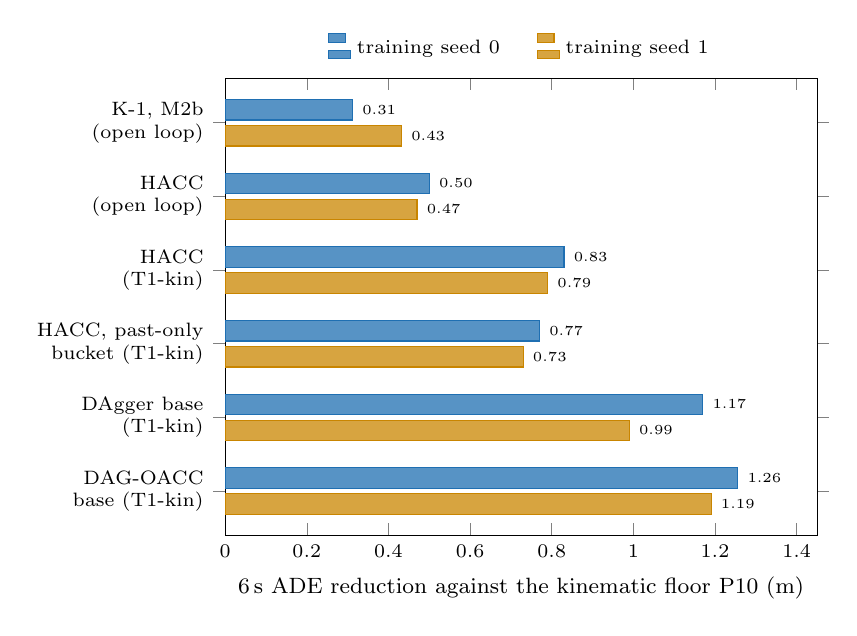
\begin{tikzpicture}
\begin{axis}[
  xbar, scale only axis, width=0.62\columnwidth, height=58mm, bar width=2.6mm,
  xmin=0, xmax=1.45, xlabel={6\,s ADE reduction against the kinematic floor P10 (m)},
  xlabel style={font=\footnotesize}, ticklabel style={font=\scriptsize},
  symbolic y coords={DAGO,DAG,HACCc,HACCt,HACCo,K1},
  ytick=data, yticklabel style={align=right},
  yticklabels={{K-1, M2b\\(open loop)},{HACC\\(open loop)},{HACC\\(T1-kin)},{HACC, past-only\\bucket (T1-kin)},{DAgger base\\(T1-kin)},{DAG-OACC\\base (T1-kin)}},
  enlarge y limits=0.12,
  legend style={font=\scriptsize,at={(0.5,1.02)},anchor=south,legend columns=2,draw=none,fill=none,/tikz/every even column/.append style={column sep=4mm}},
  nodes near coords, nodes near coords style={font=\tiny,anchor=west}, reverse legend,
  point meta=explicit symbolic,
]
\addplot[fill=levO!75,draw=levO] coordinates {(0.432,K1)[0.43] (0.47,HACCo)[0.47] (0.79,HACCt)[0.79] (0.73,HACCc)[0.73] (0.99,DAG)[0.99] (1.1903,DAGO)[1.19]};
\addplot[fill=levT!75,draw=levT] coordinates {(0.312,K1)[0.31] (0.50,HACCo)[0.50] (0.83,HACCt)[0.83] (0.77,HACCc)[0.77] (1.17,DAG)[1.17] (1.2556,DAGO)[1.26]};
\legend{training seed 1, training seed 0}
\end{axis}
\end{tikzpicture}
\caption{\textbf{Six-second error reduction against the learned kinematic floor}, at two training seeds. Every bar is a paired
episode-cluster bootstrap contrast on 141 held-out episodes, and every one is separated from zero. The tier is given per bar.}
\label{fig:bars}
\end{figure}

\begin{table}[t]
\centering
\caption{\textbf{Headline results} (MEASURED; paired episode-cluster bootstrap, $B=2000$, 141 episodes; values at seed 0 / seed 1).}
\label{tab:headline}
\small
\begin{tabularx}{\columnwidth}{@{}>{\raggedright\arraybackslash}Xl@{}}
\toprule
Result & Tier \\
\midrule
6\,s ADE $-0.312$\,/\,$-0.432$\,m vs P10, beyond the pre-registered $2F=0.2415$\,m (12.5--17.4\,\% lower error) & open loop \\
HACC post-map: better than P10 on \emph{every} row of the pre-registered set (ADE2, ADE6, accel., curvature, speed, heading, yaw rate, decisions, consistency) & open loop \\
6\,s ADE $-0.83$\,/\,$-0.79$\,m vs P10 on own executed motion; $-0.77$\,/\,$-0.73$\,m with a past-only speed bucket & T1-kin \\
Route checkpoints beat a kinematic arc by 1.2/3.3/7.8\,m and 1.3/3.5/8.8\,m at 30/50/80\,m & T1-kin \\
DAgger: tactical macro-F1 $+0.108$/$+0.118$ (lateral), $+0.055$/$+0.081$ (longitudinal); 6\,s ADE $-0.54$/$-0.40$\,m vs its control & T1-kin \\
Adopted base: 6\,s ADE $-1.26$\,/\,$-1.19$\,m vs P10; every family has a separated-better row & T1-kin \\
Per band: DAgger rows lower 2--6\,s ADE by 0.82\,/\,0.62\,m; the acceleration term lowers 0--2\,s ADE by 0.062\,/\,0.079\,m and 0--2\,s acceleration error by 0.97\,/\,1.14\,m/s$^2$ & T1-kin \\
Band loss, operative level detached: 0--2\,s ADE $-0.017$\,/\,$-0.015$\,m beyond a same-recipe replicate; no 2--6\,s row moves & T1-kin \\
Top-3 tactical manoeuvres contain the logged one in 90\,\% of windows (top-1: 57--59\,\%); best of three plans $-0.35$ to $-0.39$\,m 2--6\,s ADE (oracle) & T1-kin \\
Tactical headroom: 87\,/\,89\,\% in the continuous constraints; a forced correct stop lowers stop-point tactical ADE by 1.54\,/\,1.48\,m; stop re-weighting moves recall only along one ROC curve (oracle) & T1-kin \\
Ground-truth tactical code: 6\,s ADE from $\approx$2.1 to $\approx$1.0\,m (interface headroom) & T0 \\
\bottomrule
\end{tabularx}
\end{table}

\paragraph{The hierarchy beats its floor.} Against the learned kinematic floor P10, which is exactly the model's own output at a zero
residual by \cref{eq:traj}, v8F-mini (M2b) lowers 6\,s error by 0.312/0.432\,m at two seeds, beyond a pre-registered bar of twice the
seed floor (\cref{fig:bars}, \cref{tab:headline}). A zero-training post-map (HACC) blends O's plan with its own prior through
per-step weights fitted on training windows with an acceleration term. With it, the model is separated-better than P10 on every row of
a pre-registered set, including 2\,s error ($-0.011$/$-0.008$\,m), 6\,s error ($-0.50$/$-0.47$\,m) and acceleration
($-0.022$/$-0.040$\,m/s$^2$), and separated-worse on none.

\paragraph{The margin survives the model's own motion.} On T1-kin, where the ego state is rebuilt from the model's own executed motion at
each replan, the HACC model beats P10 by 0.83/0.79\,m. Two stress versions keep most of the margin:
\begin{itemize}
  \item a speed bucket rebuilt from the last 4\,s of measured speed alone keeps 0.77/0.73\,m;
  \item freezing the camera at the first frame for 6\,s as well keeps 0.73/0.64\,m.
\end{itemize}
The margin therefore rests on the model's reading of the scene and of its own state, not on future information.

\paragraph{On-policy data makes the tactical brain robust.} Replacing 10\,\% of training samples by the model's own rolled-out states
(DAgger, $p=0.1$) raises the tactical brain's lateral macro-F1 by 0.108/0.118 and its longitudinal macro-F1 by 0.055/0.081 on the
model's own motion. It also lowers executed 6\,s error by 0.54/0.40\,m. It is the first training lever to clear a T1 bar on both
heads. The adopted base built on it (DAG-OACC) lowers 6\,s error against P10 by 1.26/1.19\,m on its own motion. At least one row
improves in each of the four families (longitudinal, lateral, tactical and strategic).

\paragraph{Every level contributes.} The strategic brain's route checkpoints beat a kinematic arc at every horizon, by up to 8.8\,m at
80\,m. The tactical interface is used, as substituting the ground-truth code cuts 6\,s error from about 2.1 to about 1.0\,m.
\Cref{prop:lip} reads this as roughly 1.1\,m of headroom available through better tactical predictions. Because the response is
convex, that headroom concentrates in the final gains in tactical precision.

\paragraph{Which lever carries which band.} Under the band definition of \cref{sec:bands}, we retrained the operative and tactical levels with a per-band loss and with the operative level's loss detached from the tactical level, at two seeds and with a same-recipe replicate (\tier{T1-kin} throughout). The 0--2\,s plan improves at both seeds beyond the replicate: ADE by 0.017/0.015\,m, about 6\,\%, and FDE at 2\,s by 0.039/0.027\,m. No row of the 2--6\,s band moves, and the replicate says why: two runs of the same recipe differ there by 0.29\,m. A ladder of banked fine-tunes splits the adopted base into its three changes. The DAgger rows carry the tactical band (2--6\,s ADE $-0.82$/$-0.62$\,m, heading $-4.6$/$-2.6^{\circ}$). The acceleration-matching term carries the operative band and acceleration (0--2\,s ADE $-0.062$/$-0.079$\,m; acceleration error $-0.97$/$-1.14$\,m/s$^2$ at 0--2\,s and $-2.0$/$-2.6$\,m/s$^2$ at 2--6\,s). Decoding the operative level once per top-three tactical manoeuvre, the logged manoeuvre is among the three in 90\,\% of windows against 57--59\,\% for the first choice, and the best of the three plans would lower 2--6\,s ADE by 0.35--0.39\,m. That oracle gap is the measured headroom of a trained selection over the tactical codes, and the next lever.

\paragraph{Where the tactical headroom sits.} We measured that lever before building it, with zero-training oracle reads on the adopted recipe (\tier{T1-kin}, first tick, both seeds, every control at its known value; the strategic family paused). A perfect selector over the top three manoeuvres captures only 24/23\,\% of the best-of-three gain, so the choice among manoeuvres is not where the headroom lies. Writing the ground-truth tactical code in place of the model's own lowers tactical ADE by 1.63/1.77\,m. Leaving out its continuous constraints forfeits 87/89\,\% of that gain and leaving out the discrete decision 11/9\,\%; target speed is the costliest single constraint. The speed error spreads over every stratum, but stop-point windows hold 20\,\% of its squared mass on 5\,\% of the windows. There the decision misses: the goal head says stop in 10/13\,\% of the 117 stop-point windows, although its stop score separates them from the rest with AUROC 0.84/0.86. Forcing the correct stop into the tactical code lowers their tactical ADE by 1.54/1.48\,m (30--31\,\%), so the operative level executes a stop once it is decided.

Three pre-registered levers then acted on the decision alone. Hardening the model's own decision at inference recovers 3--6\,\% of that gain at a cost on the other windows, and a threshold chosen on training clips does not help. Re-weighting the stop classes at two doses raises stop recall from 0.06--0.15 to 0.45--0.62 and the false-stop rate from 0.5--1.3\,\% to 12--14.5\,\%, with AUROC unchanged within its replicate floor: the weights slide the operating point along one ROC curve and add no discrimination, and stop-point ADE does not improve beyond its 0.70\,m floor. The missing piece is discrimination, which is a perception question. Its ceiling was fixed before any training: a correct stop on the 82 of 117 stop-point windows that the model already ranks highest lowers tactical ADE there by 0.96/0.86\,m, beyond the floor at both seeds, with a separated lateral cost (yaw-rate error $+2.2^{\circ}$/s) that comes with the forced stop. Linear and small MLP probes on the frozen features rank stops no better than the model (AUROC 0.84--0.87 for every input set, a 4$\times$ finer token grid included), so the first perception arm trains instead of probing: a vision-only stop-location auxiliary loss, queued to train at two seeds against same-seed controls and two replicates. Two recipe levers closed on the way: on the DAgger base, detaching the operative level costs nothing, and the band loss's operative gain shrinks to 1--2\,mm and does not settle over four seeds.

% =====================================================================================================================
\subsection{Testing the premises of the theory}\label{sec:premises}
Each read below was pre-registered with its controls and both outcomes, and is a \tier{T0} or \tier{T1-kin} diagnostic on logged
frames; the strategic family stays paused. Three experiments are still training, and their reads are not in this version.

\paragraph{Hierarchy against a flat control (T2).} A flat control at matched budget cuts the interface between the tactical and the
operative level. On all windows, with on-policy (DAgger) data in both arms, the comparison is \emph{not established}: 6\,s ADE,
hierarchy minus flat, is $-0.345$\,m $[-0.442,-0.251]$ at seed 0 and $-0.054$\,m $[-0.161,+0.055]$ at seed 1 (\tier{T1-kin}, one run
per arm per seed). Split by window class, with the mode thresholds fixed before the read (1,305 selection-critical and 1,094
common-case windows), the hierarchy is ahead on selection-critical windows by 0.48/0.16\,m, separated at both seeds; without
on-policy data it is ahead by 0.18/0.12\,m, separated at one seed. On common-case windows it is ahead by 0.18\,m at seed 0 and behind
by 0.07\,m at seed 1 with on-policy data, and behind by 0.32/0.49\,m without. The difference between the two classes is negative and
separated in all four cells ($-0.29$, $-0.23$, $-0.50$, $-0.61$\,m). This is the pattern that \cref{prop:dom} permits: a gain where
modes separate, and none promised elsewhere. It is not yet the mechanism: an exact decomposition does not place the margin in the
selection term, and both arms miss the logged 12-cell mode on 53 to 71\,\% of windows. A commit rule does not bank the gain either.
Letting the hierarchy drive only where its tactical output is confident beats both arms in no cell, because that confidence
separates the two window classes at AUROC 0.64 only; by the break-even condition of \cref{sec:theory}, a gate at that AUROC banks an
estimated 0.3 to 7.4\,\% of what a gate with the logged class would. The lever is the accuracy of the decision, not a gate on it.
With one run per arm all of this is necessary evidence and not sufficient. The deciding experiment is training: 24 arms at six seeds, hierarchy against flat under both training protocols,
with seeds as the unit. A window class reads for the hierarchy only when all six seed differences agree in sign and the two-level
interval excludes zero.

\paragraph{A yardstick for the world model (T1, T6).} The latent features are slow: their lag correlation is 0.975 at 0.2\,s and 0.883
at 2\,s. Against a forecast of no change, the learned predictor's skill is $+0.001$ at 0.2\,s, where a cross-fitted closed-form ridge
reads $+0.022$, and $-0.15$/$-0.17$ at 2\,s, where the ridge reads $+0.12$/$+0.13$ (\tier{T0}). A closed-form stack of the ridge and
the learned prediction reads $+0.040$, $+0.06$, $+0.15$ and $+0.17$ at 0.2, 0.4, 0.8 and 2.0\,s, above both parts at every horizon and
both seeds: weights written without a gradient step improve the world model. The premise of \cref{prop:jump} holds in the linear
class and strengthens with the horizon. The direct error is 0.74, 0.57, 0.52 and 0.42 of the composed one-step bound at 0.4, 0.8, 1.0
and 2.0\,s (0.416 $[0.389,0.449]$ at 2\,s). Multi-level prediction is therefore the right structure for these latents, and the learned
ten-step rollout is the part that fails. Even the stack explains only 4 to 17\,\% of the change, so the target space limits
imagination as well.

\paragraph{Rules by construction (T3).} Unshielded plans pass the logged rest point in 91.6/84.7\,\% of the 131 stop windows. The
verified shield, given the logged rest distance (a privileged ceiling), brings the overrun to exactly zero on every feasible window
and lowers stop-window 2--6\,s ADE by 3.51/3.37\,m with no cost in any cell (\tier{T1-kin}). Given the stop position that the model
itself emits (median error 11.8/9.6\,m, a flag on 10/18 of the 131 windows) it gains nothing. A split-conformal margin behaves as
proved, with held-out coverage 0.908 for a nominal 0.9, at the price of a margin of about 7.4\,m. Probes on the frozen tokens do not
supply the cue: ego kinematics alone rank stops at AUROC 0.810 $[0.744,0.868]$, and adding the $8\times20$ tokens changes that by
$-0.011$ $[-0.061,+0.043]$ (the stop label is derived from logged ego motion, so the ego baseline partly reads the source of its
own label). Rule adherence comes from the construction; usefulness comes from the sharpness of the cue.

\paragraph{A class weight is one number (T4).} Adding one scalar to the stop-goal bias of the unweighted model reproduces what a full
training run with a stop class weight does to the stop decision. At the offset that matches the trained false-positive rate, the hit rate
is within the replicate gap of the trained arm in all four cells (differences 0.009--0.026 against a gap of 0.068), and the stop
AUROC stays at 0.819/0.850 (\tier{T1-kin}, first tick). A dose is an edit that costs seconds; a better stop decision needs a better cue.

\paragraph{What the camera interface carries (T5).} The frozen tokens carry non-ego content beyond ego motion on four targets
(\tier{T0}, 139 episodes): lead gap $+0.29$ $R^2$ $[+0.11,+0.55]$, nearest agent $+0.15$, agent count $+0.16$ and lead presence $+0.18$
AUROC $[+0.09,+0.27]$. A prediction of ours failed here. From the camera geometry we had expected that no reader of the $4\times10$
tokens recovers far range; measured, they carry range beyond ego motion in the far stratum, and under a rank-256 probe an $8\times20$
grid adds nothing (lead gap $+0.011$ $R^2$ $[-0.023,+0.048]$). The probe rank hid part of the answer: with a full-kernel probe the
finer grid is ahead by $+0.076$ $R^2$ $[+0.001,+0.170]$ on lead gap and $+0.043$ AUROC $[+0.022,+0.066]$ on lead presence. Read
directly with an attentive probe, un-pooled $16\times40$ tokens give lead gap $R^2$ 0.46, against 0.40 for the $4\times10$ grid and 0.13
for ego motion alone; the best fine set gains $+0.055$ $[+0.000,+0.111]$, under its bar of 0.10, and lead presence rises from AUROC
0.77 to 0.84 ($+0.066$ $[+0.033,+0.103]$). The probes are still rising at 111 training episodes, so these reads are lower bounds.
A finer interface is a live but thin lever; the larger gap lies between what the tokens carry and what the model's own state exposes.

\paragraph{The world-model state, untrained and trained (T5, T7).} \Cref{prop:pool} was written before its controls. On real tokens a
planted object's position is read at AUROC 1.000 from a state that keeps the cell layout and 0.495 from the mean state, and a planted
motion at 1.000 from two frames of the grid state and 0.493 from two frames of the mean state. Without training, the lead gap is read
at $R^2$ 0.40 from the grid state, 0.26 from the mean state and 0.13 from ego motion alone; grid minus ego is $+0.27$ $[+0.08,+0.54]$,
and grid minus mean, $+0.14$ $[-0.004,+0.29]$, does not exclude zero on 139 episodes. On the \emph{trained} model the mean state was read at
two training seeds. Out of sample it tells whether a lead vehicle is present at AUROC 0.807/0.788, against 0.596 from ego motion
(differences $+0.211$ $[+0.105,+0.314]$ and $+0.192$ $[+0.101,+0.286]$). On 1,200 training clips it reads the lead gap at $R^2$ 0.456/0.445
against 0.187. For the \emph{change} of that gap over 2\,s, ego motion alone has a skill of $+0.291$ over persistence, and adding the
state adds nothing: $-0.028$ $[-0.065,+0.008]$ and $-0.025$ $[-0.059,+0.009]$. The two training runs differ by 0.010 in gap $R^2$. The
trained state knows where the lead is, and nothing about where it is going beyond ego motion: \cref{prop:pool} on a trained model.
Decoded back to pictures, the state shows the scene gist (sky, road, light level) and no object, at a skill of 0.36/0.35 against 0.78
for the token grid, and its learned 2\,s rollout is no closer to the true future frame than the present frame. By T7, imagination is
admissible for the gist and not for objects. Four arms are training: a state that keeps the cell layout, and a mean state of equal
width as its control, at two seeds each.

\paragraph{Weight space (T9).} The 50/50 weight average of two same-initialisation replicates lowers tactical ADE by 0.075\,m
$[0.047,0.103]$ against the member mean and realises $\kappa=0.74$ $[0.48,0.99]$ of the gain of an output ensemble, in one forward pass
and with no separated cost in any family (\tier{T1-kin}). It is not ahead of the better member; what it removes is the risk of the
worse one. Read in weight space (one replicate pair, no interval), a stop class weight moves the model less than a change of seed does in every module group, and
clearly exceeds seed noise only in two head biases, which is what T4 says a class weight is.

\paragraph{Data (T8).} At the probe level, choosing 25 or 50\,\% of the training episodes by coverage or by leverage in token space
lands inside the range of 20 random draws, so no selection claim is made for this representation. A data-efficiency experiment is
training: the same model on 1/2, 1/4 and 1/8 of the clips at fixed steps, flat against hierarchy at 1/4, and clips chosen by their
share of selection-critical windows against random clips.

\section{The frontier: assertive launch, and re-rendered simulation}\label{sec:frontier}
With the feasibility post-step, the adopted composite meets every row of the 19-row pre-registered set but one: the \emph{launch-crawl}
share. These are situations where the human pulls away from near-standstill above 5.2\,m/s and the model starts more cautiously.
Every zero-training lever available on CPU has been measured against this row:
\begin{itemize}
  \item decode levers;
  \item a level-from-image head;
  \item four doses of an external progress floor.
\end{itemize}
Even with the exact human speed supplied as a ceiling diagnostic, a bounded floor closes about half of the gap.

The analysis points to a property of the tier rather than of the planner. Logged cameras cannot show a lagging car its own
consequences: the lead vehicle never pulls away on screen, and the scene never moves at the car's own pace.

\paragraph{T2 re-perception.} The re-rendered evaluation tier runs on neural reconstructions of real drives:
\begin{itemize}
  \item 62 scenes (42 launch, 20 guard), selected by a rule frozen \emph{before} any log was read, and staged (35.7\,GB);
  \item a harness that reproduces the T1-kin plans bit for bit from cached features, with an in-loop encoder that reproduces the
        cached tokens to 2.6\,\% relative $L_2$ (cosine 0.99965).
\end{itemize}
The pre-registered design runs two conditions with the same renderer: cameras rendered at the car's \emph{own} pose and time, and at
the \emph{logged} pose re-indexed by the car's progress. Their contrast measures the camera-clock effect directly, free of the
render domain gap, and both outcomes and their next levers are committed in advance. First reads now exist on 48 scenes with replayed
traffic. An encoder adapted to the render gap improves speed error at both seeds, does not separate 6\,s error from the unadapted model at
either seed, and is not better than the floor on every row, so the launch row stays open.

% =====================================================================================================================
\section{Outlook and research roadmap}\label{sec:outlook}
\begin{table}[t]
\centering
\caption{\textbf{Roadmap} (\emph{outlook}: not yet implemented unless marked).}
\label{tab:roadmap}
\small
\begin{tabularx}{\columnwidth}{@{}>{\raggedright\arraybackslash}p{24mm}>{\raggedright\arraybackslash}X@{}}
\toprule
Item & What it delivers \\
\midrule
T2 re-perception \textit{(first reads, 48 scenes)} & a decision-grade read of the launch row on re-rendered scenes; the longitudinal tier for every later arm \\
World-model planner \textit{(built)} & top-down planning over three latent levels, the baseline for comparing other approaches; its first gates on the M2b latents do not yet beat holding the logged action (\tier{T0}); giving its predictor the measured speed does not raise its skill beyond the seed floor (\tier{T0}); a slow-feature basis is being read \\
Band retraining \textit{(read, four seeds)} & on the DAgger base the detach costs nothing; the band loss's 1--2\,mm operative gain does not settle, so it is closed as a recipe lever \\
Tactical selection \textit{(oracle read)} & a perfect top-3 selector captures 24/23\,\% of the best-of-three headroom; the headroom sits in the speed constraint, so no selector is built \\
Stop perception \textit{(queued, two seeds)} & a vision-only stop-location auxiliary on the tactical level; measured ceiling 0.86--0.96\,m tactical ADE on stop-point windows (oracle) \\
Strategic context labels \textit{(in production)} & per-frame country, period of day, illumination, weather, visibility, road surface \\
Perception adaptation \textit{(in training, seed 0)} & LoRA on the visual encoder for motion cues; about 184\,h per seed on the 20\,GB pod GPU at the measured 34.5\,s per step \\
Scale data & from 4,512 clips toward the full corpus; on-policy DAgger data from T2 rollouts \\
Scale size & from 7\,M toward the 4B budget of at most 800\,M, with each level's predictor in its own latent \\
Strategic topology & routing over a latent transition graph, with map structure from simulation or an external corpus \\
Fallback brain & imagination-error monitoring, the minimal-risk manoeuvre and ISMR/DSSAD logging \\
Occlusion imagination & multi-step, calibrated belief roll-out of hidden sectors \\
Edge deployment & Jetson Thor, at most 100\,ms end to end on 4 cameras \\
Benchmarks & NAVSIM navtest and pre-registered T2 reads \\
\bottomrule
\end{tabularx}
\end{table}

The roadmap (\cref{tab:roadmap}) follows from the measurements. The architecture is validated at small scale on a consumer GPU,
every level carries measurable value, and the remaining behaviour sits where logged-camera evaluation cannot see. Three investments
turn the validated design into a driver:
\begin{itemize}
  \item a \textbf{re-rendered simulation tier}, with first reads in hand;
  \item \textbf{perception adaptation} for motion and stop cues;
  \item \textbf{scale in data and model size} toward the 4B budget.
\end{itemize}
Because the floor identity holds at every scale, and every lever is pre-registered with deliberate-regression controls, each
investment yields a measured answer rather than an anecdote.

The theory of \cref{sec:theory} orders the next steps. Three experiments are training on one GPU: the six-seed replicate that
decides the hierarchy against its flat control; a world-model state that keeps the cell layout, which by \cref{prop:pool} is the
least change that lets the state hold where an object is and how it moves; and the data-efficiency curve that says whether the
next limit is data. The premise of \cref{prop:dom} for v8F-mini is the next read: selection accuracy against the share of the
larger mode per context.

% =====================================================================================================================
\section{Conclusion}
TanitAD-4B drives at every level of abstraction and holds every level accountable. Its reference implementation shows that a typed
hierarchy over frozen foundation features clears a learned kinematic floor:
\begin{itemize}
  \item in open loop, by 0.31--0.43\,m of 6\,s error;
  \item on every row of a pre-registered set, with a zero-training post-map;
  \item on its own executed motion, by more than a metre, with at least one improved row in each of the four metric families.
\end{itemize}
It does so with 7.2\,M trainable parameters and four GPU-hours. The mathematics explains where the remaining headroom sits: in
tactical precision, with convex returns, and in the evaluation tier. A machine-checked theory states when the hierarchy can
dominate and what its present world-model state cannot hold, and the measurements place v8F-mini against each premise: ahead
where modes separate, not yet established overall, and limited by a pooled state that keeps the scene and loses its objects. The roadmap names the investments that will convert the
architecture into a deployable, self-aware driver.

\paragraph{Acknowledgements.} Experiments, instruments and reports were produced with the TanitAD autonomous research system under
the author's direction.

% =====================================================================================================================
\begin{thebibliography}{99}\footnotesize\setlength{\itemsep}{0.5pt}\setlength{\parsep}{0pt}
\bibitem{hjepa} H-JEPA: Hierarchical joint-embedding predictive world models. arXiv:2610.06805, 2026.
\bibitem{hplwm} Hierarchical planning with latent world models. arXiv:2604.03208, 2026.
\bibitem{orbis2} Orbis 2. arXiv:2607.15898, 2026.
\bibitem{drivehwm} Drive-HWM: slow and fast world models for driving. arXiv:2609.03572, 2026.
\bibitem{s2planner} S2Planner: a multi-scale semantic planner. arXiv:2609.29813, 2026.
\bibitem{dinov3} O.~Sim\'eoni et al. DINOv3. arXiv:2508.10104, 2025.
\bibitem{vjepa2} M.~Assran et al. V-JEPA~2: Self-supervised video models enable understanding, prediction and planning. arXiv:2506.09985, 2025.
\bibitem{lejepa} R.~Balestriero and Y.~LeCun. LeJEPA: Provable and scalable self-supervised learning without the heuristics. arXiv:2511.08544, 2025.
\bibitem{lora} E.~J.~Hu et al. LoRA: Low-rank adaptation of large language models. arXiv:2106.09685, 2021.
\bibitem{ssshashua} S.~Shalev-Shwartz and A.~Shashua. On the sample complexity of end-to-end training vs.\ semantic abstraction training. arXiv:1604.06915, 2016.
\bibitem{schedsamp} S.~Bengio, O.~Vinyals, N.~Jaitly and N.~Shazeer. Scheduled sampling for sequence prediction with recurrent neural networks. arXiv:1506.03099, 2015.
\bibitem{dagger} S.~Ross, G.~Gordon and J.~A.~Bagnell. A reduction of imitation learning and structured prediction to no-regret online learning. arXiv:1011.0686, 2011.
\bibitem{dart} M.~Laskey et al. DART: Noise injection for robust imitation learning. arXiv:1703.09327, 2017.
\bibitem{causalconf} P.~de~Haan, D.~Jayaraman and S.~Levine. Causal confusion in imitation learning. arXiv:1905.11979, 2019.
\bibitem{bclimits} F.~Codevilla et al. Exploring the limitations of behavior cloning for autonomous driving. arXiv:1904.08980, 2019.
\bibitem{cil} F.~Codevilla et al. End-to-end driving via conditional imitation learning. arXiv:1710.02410, 2018.
\bibitem{chauffeurnet} M.~Bansal, A.~Krizhevsky and A.~Ogale. ChauffeurNet: Learning to drive by imitating the best and synthesizing the worst. arXiv:1812.03079, 2018.
\bibitem{transfuser} K.~Chitta et al. TransFuser: Imitation with transformer-based sensor fusion for autonomous driving. arXiv:2205.15997, 2022.
\bibitem{vad} B.~Jiang et al. VAD: Vectorized scene representation for efficient autonomous driving. arXiv:2303.12077, 2023.
\bibitem{hydramdp} Z.~Li et al. Hydra-MDP: End-to-end multimodal planning with multi-target hydra-distillation. arXiv:2406.06978, 2024.
\bibitem{diffusiondrive} B.~Liao et al. DiffusionDrive: Truncated diffusion model for end-to-end autonomous driving. arXiv:2411.15139, 2024.
\bibitem{resad} ResAD: normalised residual trajectory modelling for end-to-end driving. arXiv:2510.08562, 2025.
\bibitem{navsim} D.~Dauner et al. NAVSIM: Data-driven non-reactive autonomous vehicle simulation and benchmarking. arXiv:2406.15349, 2024.
\bibitem{nuplan} N.~Karnchanachari et al. Towards learning-based planning: The nuPlan benchmark for real-world autonomous driving. arXiv:2403.04133, 2024.
\bibitem{nachum18} O.~Nachum, S.~Gu, H.~Lee and S.~Levine. Near-optimal representation learning for hierarchical reinforcement learning. arXiv:1810.01257, 2018.
\bibitem{nachum19} O.~Nachum et al. Why does hierarchy (sometimes) work so well in reinforcement learning? arXiv:1909.10618, 2019.
\bibitem{mbpo} M.~Janner, J.~Fu, M.~Zhang and S.~Levine. When to trust your model: Model-based policy optimization. arXiv:1906.08253, 2019.
\end{thebibliography}

\end{document}
